\documentclass[journal]{IEEEtran}
\usepackage[a5paper, margin=10mm]{geometry}
%\usepackage{lmodern} % Ensure lmodern is loaded for pdflatex
\usepackage{tfrupee} % Include tfrupee package

\setlength{\headheight}{1cm}
\setlength{\headsep}{0mm}

\usepackage{gvv-book}
\usepackage{gvv}
\usetikzlibrary{patterns}
\lstset{aboveskip=12pt}
\usepackage[center]{caption}
\raggedbottom

\hypersetup{
    colorlinks=true,
    urlcolor=black
}
\usepackage{amsfonts}
\makeindex

\begin{document}
\bibliographystyle{IEEEtran}
\onecolumn

\title{
    \begin{center}
        Math for EE
        \\
        \rule{0.4\columnwidth}{0.4pt}
    \end{center}
}
\author{
    \vspace{11cm}
    \begin{center}
        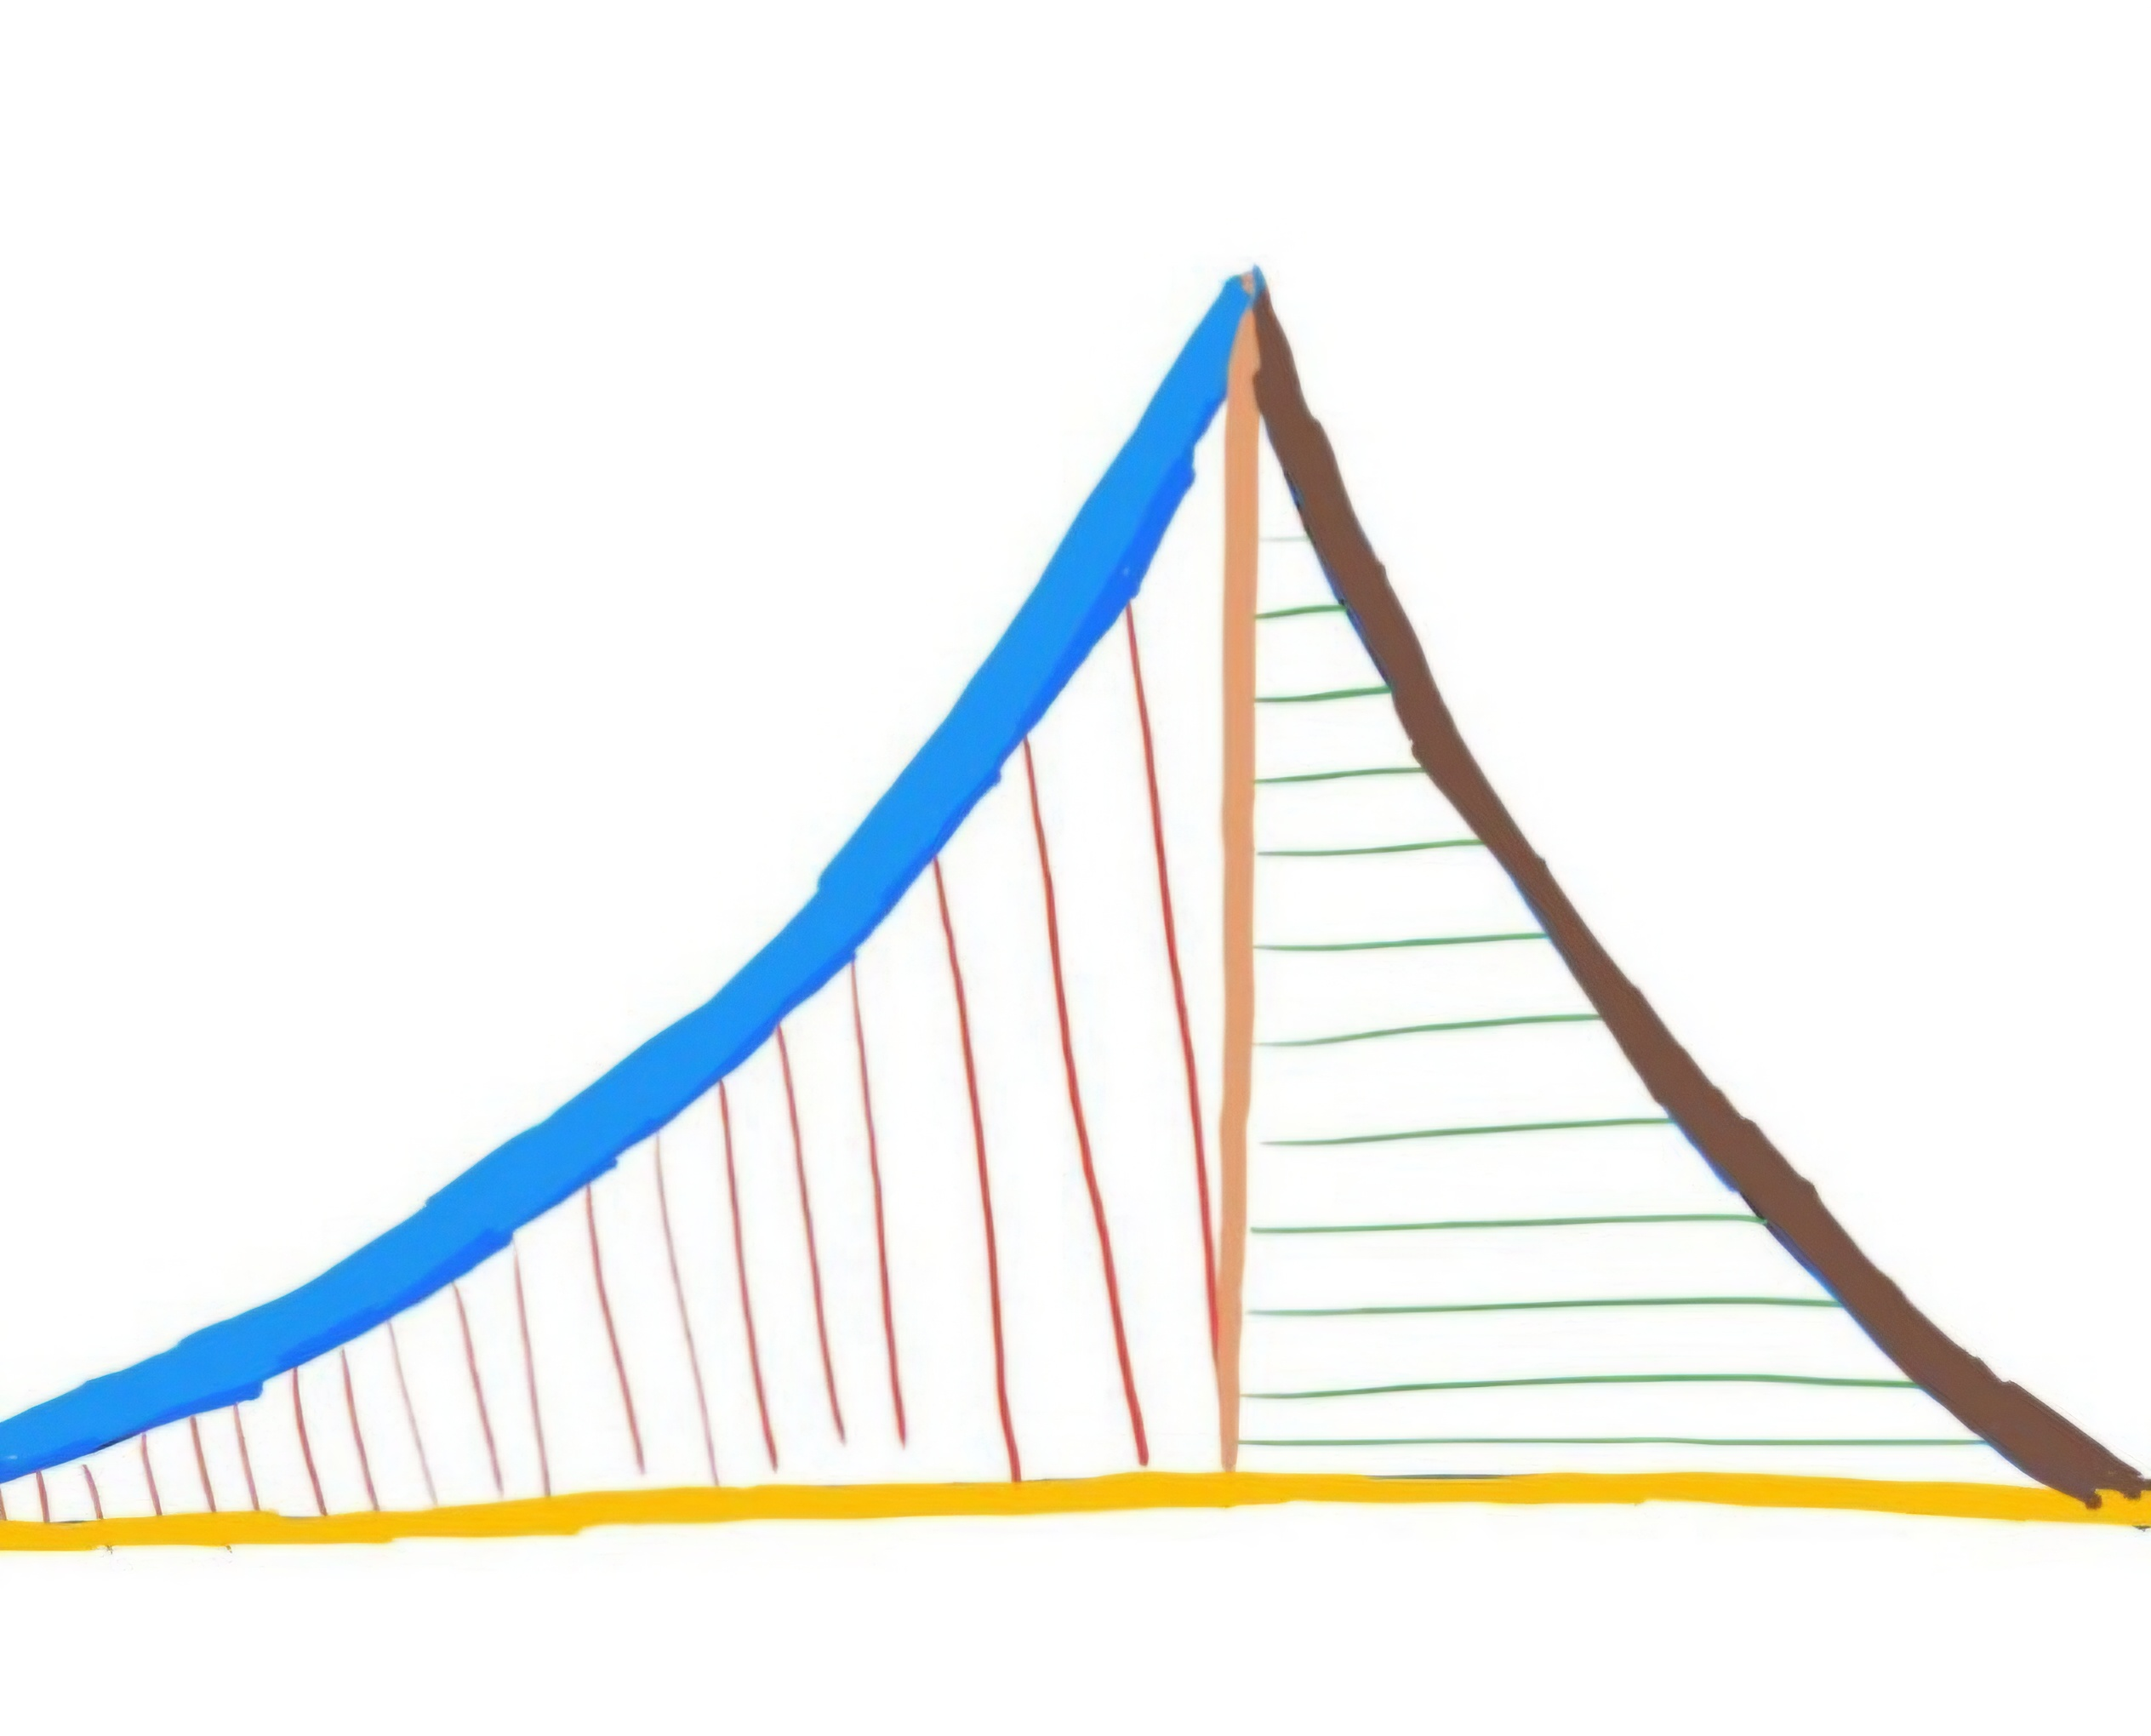
\includegraphics[width=0.2\columnwidth]{figs/logo.jpg}
        \\
        {\huge G. V. V. Sharma}
    \end{center}
}
\maketitle

\newpage
\section*{About this Book}

This book introduces matrices through high school coordinate geometry.
This approach makes it easier for beginners to learn Python for scientific
computing. All problems in the book are from NCERT mathematics textbooks
from Class 9--12. Exercises are from CBSE board exam papers.

The content is sufficient for industry jobs and covers nearly all matrix
prerequisites for machine learning. There is no copyright, so readers are
free to print and share.
License: https://creativecommons.org/licenses/by-sa/3.0/
\\
and
\\
https://www.gnu.org/licenses/fdl-1.3.en.html
\\
First manual appeared in January 2018
\\
First edition published on July 10, 2024
\\
In this edition, some incorrect solutions were removed. All figures
redrawn. More problems added.

\newpage
\onecolumn
\begin{center}
{\Large\bfseries CBSE 2026 12th class maths solutions (65-3-1)}
\end{center}
\vspace{0.4em}

\begin{list}{}{\setlength{\leftmargin}{1.15cm}\setlength{\labelwidth}{1.0cm}\setlength{\labelsep}{0.15cm}\setlength{\itemindent}{0pt}\setlength{\listparindent}{0pt}\setlength{\itemsep}{\baselineskip}\setlength{\parsep}{0pt}\setlength{\topsep}{0pt}}
\item[3.1.2] If $A^2=4A+3I$ and $A^{-1}=xA+yI$, find $x+y$.

\noindent (A) $-1$ \hfill (B) $1$ \hfill (C) $\frac53$ \hfill (D) $7$

\vspace{0.6em}\par\noindent\textbf{Solution:}

Multiply $A^2=4A+3I$ by $A^{-1}$. Since $A$ is invertible,
\[
A=4I+3A^{-1},\qquad A^{-1}=\frac13A-\frac43I.
\]
Comparing with $A^{-1}=xA+yI$, we get $x=\frac13$ and $y=-\frac43$. Hence
\[
x+y=\frac13-\frac43=-1.
\]
Therefore, the correct answer is \textbf{(A)}.
\item[3.1.4] If $\begin{bmatrix}4\\1\\3\end{bmatrix}A=\begin{bmatrix}-4&8&4\\-1&2&1\\-3&6&3\end{bmatrix}$, find the order of $A$.

\noindent (A) $3\times1$ \hfill (B) $1\times3$ \hfill (C) $1\times1$ \hfill (D) $3\times3$

\vspace{0.6em}\par\noindent\textbf{Solution:}

The left matrix has order $3\times1$ and the product has order $3\times3$. Hence $A$ must have one row and three columns: $\boxed{1\times3}$, option \textbf{(B)}. The C program checks all four proposed orders against matrix multiplication rules.
\begin{lstlisting}[frame=single, basicstyle=\rmfamily, escapeinside={(*@}{@*)}]
(*@\makebox[\dimexpr\linewidth-2\fboxsep-2\fboxrule\relax][c]{codes/3.1.4.c}@*)
\end{lstlisting}

\item[3.1.5] If a square matrix $A$ satisfies $A^2=A$ and $(I-A)^3=xA+I$, find $x$.

\vspace{0.6em}\par\noindent\textbf{Solution:}

Using $A^2=A$ also gives $A^3=A$. Therefore $(I-A)^3=I-3A+3A^2-A^3=I-A$. Comparing with $xA+I$ gives $x=-1$. Thus $\boxed{x=-1}$.

\item[3.1.6] If $B(\operatorname{adj}B)=\begin{bmatrix}\frac13&0&0\\0&\frac13&0\\0&0&\frac13\end{bmatrix}$, find $\det(B^{-1})$.

\vspace{0.6em}\par\noindent\textbf{Solution:}

For a $3\times3$ matrix, $B(\operatorname{adj}B)=\det(B)I$. Hence $\det(B)=\frac13$, and $\det(B^{-1})=1/\det(B)=\boxed{3}$. The Python code evaluates this determinant relation.
\begin{lstlisting}[frame=single, basicstyle=\rmfamily, escapeinside={(*@}{@*)}]
(*@\makebox[\dimexpr\linewidth-2\fboxsep-2\fboxrule\relax][c]{codes/3.1.6.py}@*)
\end{lstlisting}

\item[3.1.7] Find $k$ such that $f(x)=\begin{cases}x^2\sin(1/x),&x\ne0,\\k(x+1),&x=0\end{cases}$ is continuous.

\vspace{0.6em}\par\noindent\textbf{Solution:}

At $x=0$, the second branch gives $f(0)=k$. Also $|x^2\sin(1/x)|\le x^2$, so $\lim_{x\to0}x^2\sin(1/x)=0$. Continuity requires $k=0$. The plot shows the oscillations shrinking to the point $(0,0)$.
\begin{lstlisting}[frame=single, basicstyle=\rmfamily, escapeinside={(*@}{@*)}]
(*@\makebox[\dimexpr\linewidth-2\fboxsep-2\fboxrule\relax][c]{codes/3.1.7.py}@*)
\end{lstlisting}
\begin{figure}[H]\centering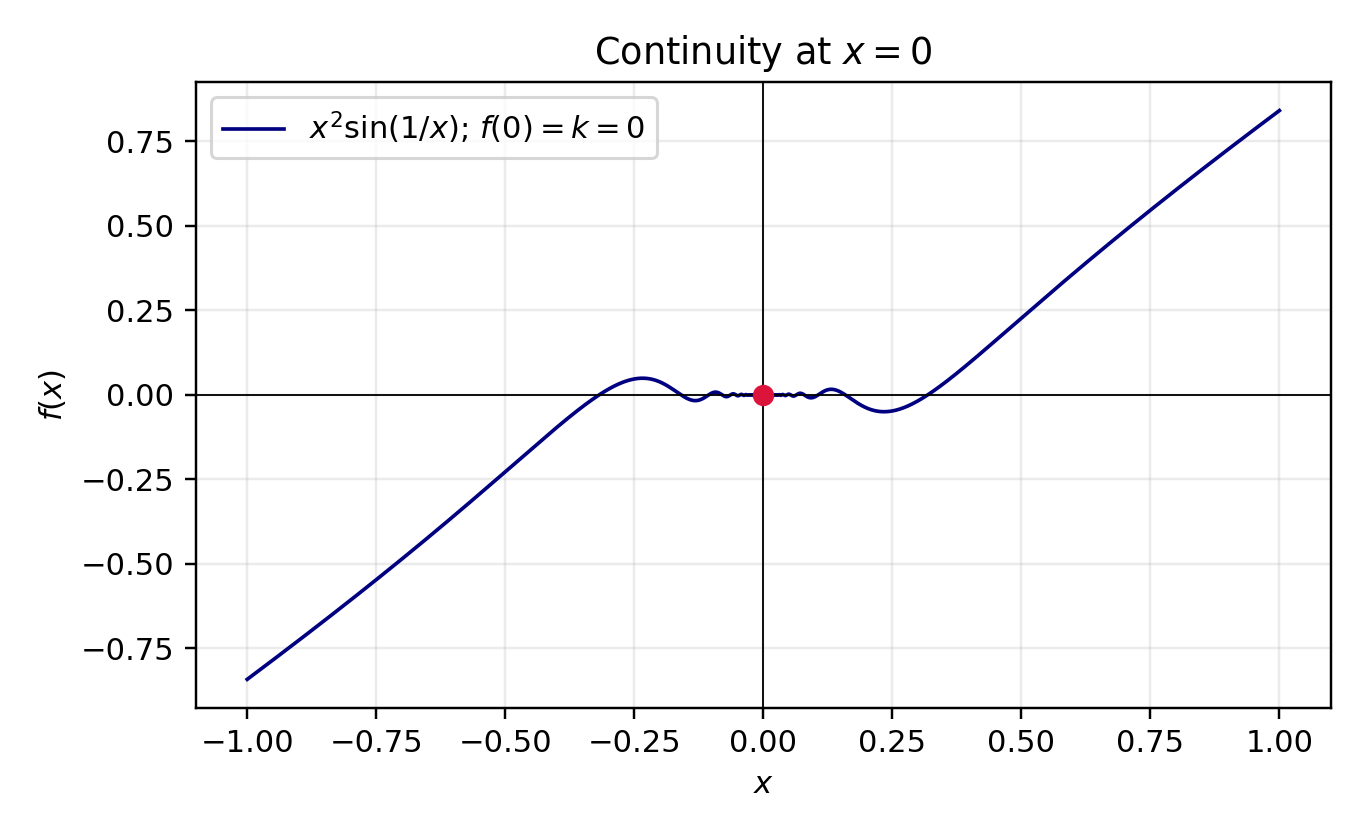
\includegraphics[width=0.68\linewidth]{figs/3.1.7.png}\caption{The function approaches $0$ as $x$ approaches $0$.}\end{figure}

\item[3.1.10] Evaluate $\displaystyle\int\frac{dx}{2^x+2^{-x}}$.

\vspace{0.6em}\par\noindent\textbf{Solution:}

Let $u=2^x$, so $dx=du/(u\ln2)$. Then
\[
\int\frac{dx}{2^x+2^{-x}}=\frac1{\ln2}\int\frac{du}{1+u^2}
=\boxed{\frac{\tan^{-1}(2^x)}{\ln2}+C}.
\]

\item[3.1.11] Evaluate $\displaystyle\int_{-1}^{1}(1-|x|)\,dx$ by identifying the matching option:

\noindent (A) $2\int_0^1(1+x)\,dx$ \hfill (B) $2\int_{-1}^0(1+x)\,dx$\\
(C) $0$ \hfill (D) $2\int_{-1}^0(1-x)\,dx$

\vspace{0.6em}\par\noindent\textbf{Solution:}

The integrand is even, and for $0\le x\le1$ it equals $1-x$. Thus the integral is $2\int_0^1(1-x)\,dx=1$. Option (B) is equivalent after the substitution $x\mapsto -x$, so the answer is \textbf{(B)}.

\item[3.1.12] For the circle $x^2+y^2=9$, identify the integral for the shaded cap above $y=1$.

\noindent (A) $\int_1^3\sqrt{9-y^2}\,dy$ \hfill (B) $2\int_1^3\sqrt{9-y^2}\,dy$\\
(C) $\int_0^3\sqrt{9-x^2}\,dx$ \hfill (D) $2\int_0^3\sqrt{9-x^2}\,dx$

\vspace{0.6em}\par\noindent\textbf{Solution:}

At a fixed height $y$, the cap runs horizontally from $x=-\sqrt{9-y^2}$ to $x=\sqrt{9-y^2}$. Its width is $2\sqrt{9-y^2}$ and $1\le y\le3$, so its area is $\boxed{2\int_1^3\sqrt{9-y^2}\,dy}$, option \textbf{(B)}.

\item[3.1.13] Which of the following functions $F(x,y)$ make $dy/dx=F(x,y)$ a homogeneous differential equation?
\[
\text{(i) }3x+2y,\quad \text{(ii) }\sin(y/x)+\log y-\log x,\quad
\text{(iii) }e^{y/x}+1,\quad \text{(iv) }\sqrt{x^2+y^2}-y.
\]
(A) (i),(ii) \quad (B) (i),(ii),(iii) \quad (C) (ii),(iii),(iv) \quad (D) (ii),(iii)

\vspace{0.6em}\par\noindent\textbf{Solution:}

A homogeneous right-hand side must depend only on $y/x$. Expression (i) is degree one, not degree zero; (ii) simplifies to $\sin(y/x)+\log(y/x)$; (iii) is already a function of $y/x$; and (iv) is homogeneous of degree one, not a function of the ratio alone. Therefore the answer is \textbf{(D), (ii) and (iii)}.

\item[3.1.15] If $(\vec a+\vec b)\cdot(\vec a-\vec b)=198$ and $|\vec a|=10|\vec b|$, select the true statement.

\noindent (A) $|\vec a|=\sqrt2$ \hfill (B) $|\vec b|=\sqrt2$ \hfill
(C) $|\vec b|=10\sqrt2$ \hfill (D) $|\vec a|=10/\sqrt2$

\vspace{0.6em}\par\noindent\textbf{Solution:}

The dot product equals $|\vec a|^2-|\vec b|^2$. Let $|\vec b|=r$, so $|\vec a|=10r$. Then $99r^2=198$, giving $r=\sqrt2$. Hence the answer is \textbf{(B)}.

\item[3.1.18] Independent events $E,F$ satisfy $P(E)=3/10$ and $P(E\cup F)=1/2$. Find $P(E|F)-P(F|E)$.

\noindent (A) $2/7$ \hfill (B) $3/35$ \hfill (C) $1/70$ \hfill (D) $1/7$

\vspace{0.6em}\par\noindent\textbf{Solution:}

Let $P(F)=p$. Independence gives $1/2=3/10+p-(3/10)p$, hence $p=2/7$. Also $P(E|F)=3/10$ and $P(F|E)=2/7$. Their difference is $3/10-2/7=\boxed{1/70}$, option \textbf{(C)}.

\item[3.1.19] Assertion (A): One particular solution of $dy/dx=e^{x+y}$ can be $e^x+e^{-y}=-2$. Reason (R): $e^x+e^{-y}=C$ is the general solution.

\vspace{0.6em}\par\noindent\textbf{Solution:}

The left side of the asserted particular solution is positive for real $x,y$, so it cannot equal $-2$; the assertion is false. Differentiating $e^x+e^{-y}=C$ gives $e^x-e^{-y}y'=0$, hence $y'=e^{x+y}$, so the reason is true. The correct choice is \textbf{(D)}.

\item[3.1.22] Find the sub-interval(s) of $(0,\pi/2)$ in which $f(x)=\tan x-4x$ is increasing.

\vspace{0.6em}\par\noindent\textbf{Solution:}

$f'(x)=\sec^2x-4>0$ precisely when $\cos x<1/2$ on this domain. Thus $f$ is increasing on $\boxed{(\pi/3,\pi/2)}$. The Python code plots the function and marks this interval.
\begin{lstlisting}[frame=single, basicstyle=\rmfamily, escapeinside={(*@}{@*)}]
(*@\makebox[\dimexpr\linewidth-2\fboxsep-2\fboxrule\relax][c]{codes/3.1.22.py}@*)
\end{lstlisting}
\begin{figure}[H]\centering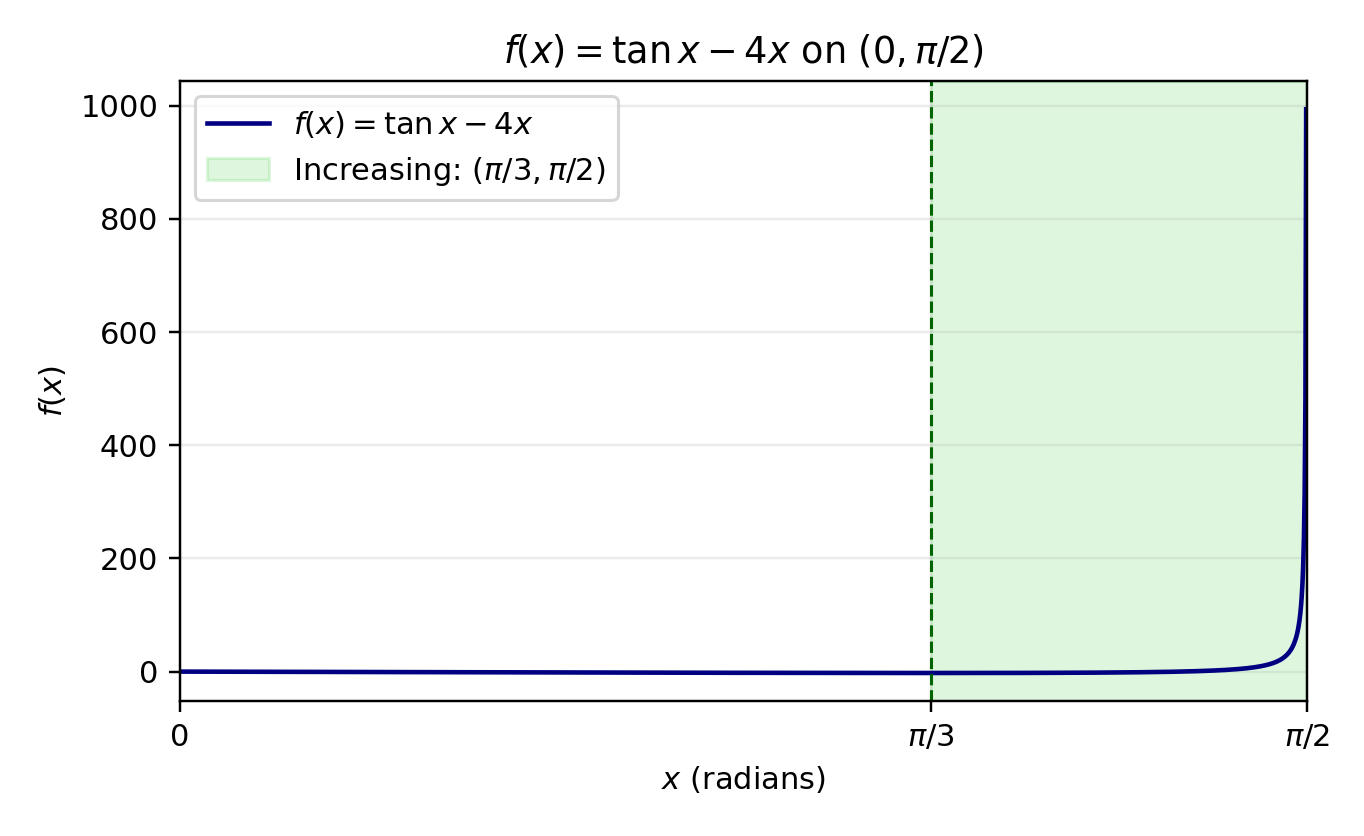
\includegraphics[width=0.68\linewidth]{figs/3.1.22.png}\caption{The function rises on the shaded interval.}\end{figure}

\item[3.1.24] For unit vectors $\vec a,\vec b$, if $|\vec a+2\vec b|=|2\vec a-\vec b|$, find the angle between them.

\vspace{0.6em}\par\noindent\textbf{Solution:}

Squaring both sides and using $|\vec a|=|\vec b|=1$ gives $5+4\vec a\cdot\vec b=5-4\vec a\cdot\vec b$, so $\vec a\cdot\vec b=0$. The angle is $\boxed{90^\circ}$.

\item[3.1.25]
(a) If $\frac{x-3}{1}=\frac{1-y}{1}=\frac{z+2}{p}$ and $\frac{2-x}{3}=\frac{y+1}{5}=\frac{z+56}{2p}$ are perpendicular, find $p$.\\
\textbf{OR}\\
(b) Find the vector equation of the line through the origin perpendicular to both $\vec r=2\hat i-\hat j+2\hat k+\lambda(3\hat i+4\hat j+2\hat k)$ and $\vec r=\mu(\hat i-\hat j+\hat k)$.

\vspace{0.6em}\par\noindent\textbf{Solution:}

(a) The direction vectors are $(1,-1,p)$ and $(-3,5,2p)$. Their dot product is $2p^2-8$, so $\boxed{p=\pm2}$.\\
(b) A suitable direction is $(3,4,2)\times(1,-1,1)=(6,-1,-7)$. The required line is $\boxed{\vec r=t(6\hat i-\hat j-7\hat k)}$. The Python code plots both alternatives and computes the direction cross product.
\begin{lstlisting}[frame=single, basicstyle=\rmfamily, escapeinside={(*@}{@*)}]
(*@\makebox[\dimexpr\linewidth-2\fboxsep-2\fboxrule\relax][c]{codes/3.1.25.py}@*)
\end{lstlisting}
\begin{figure}[H]\centering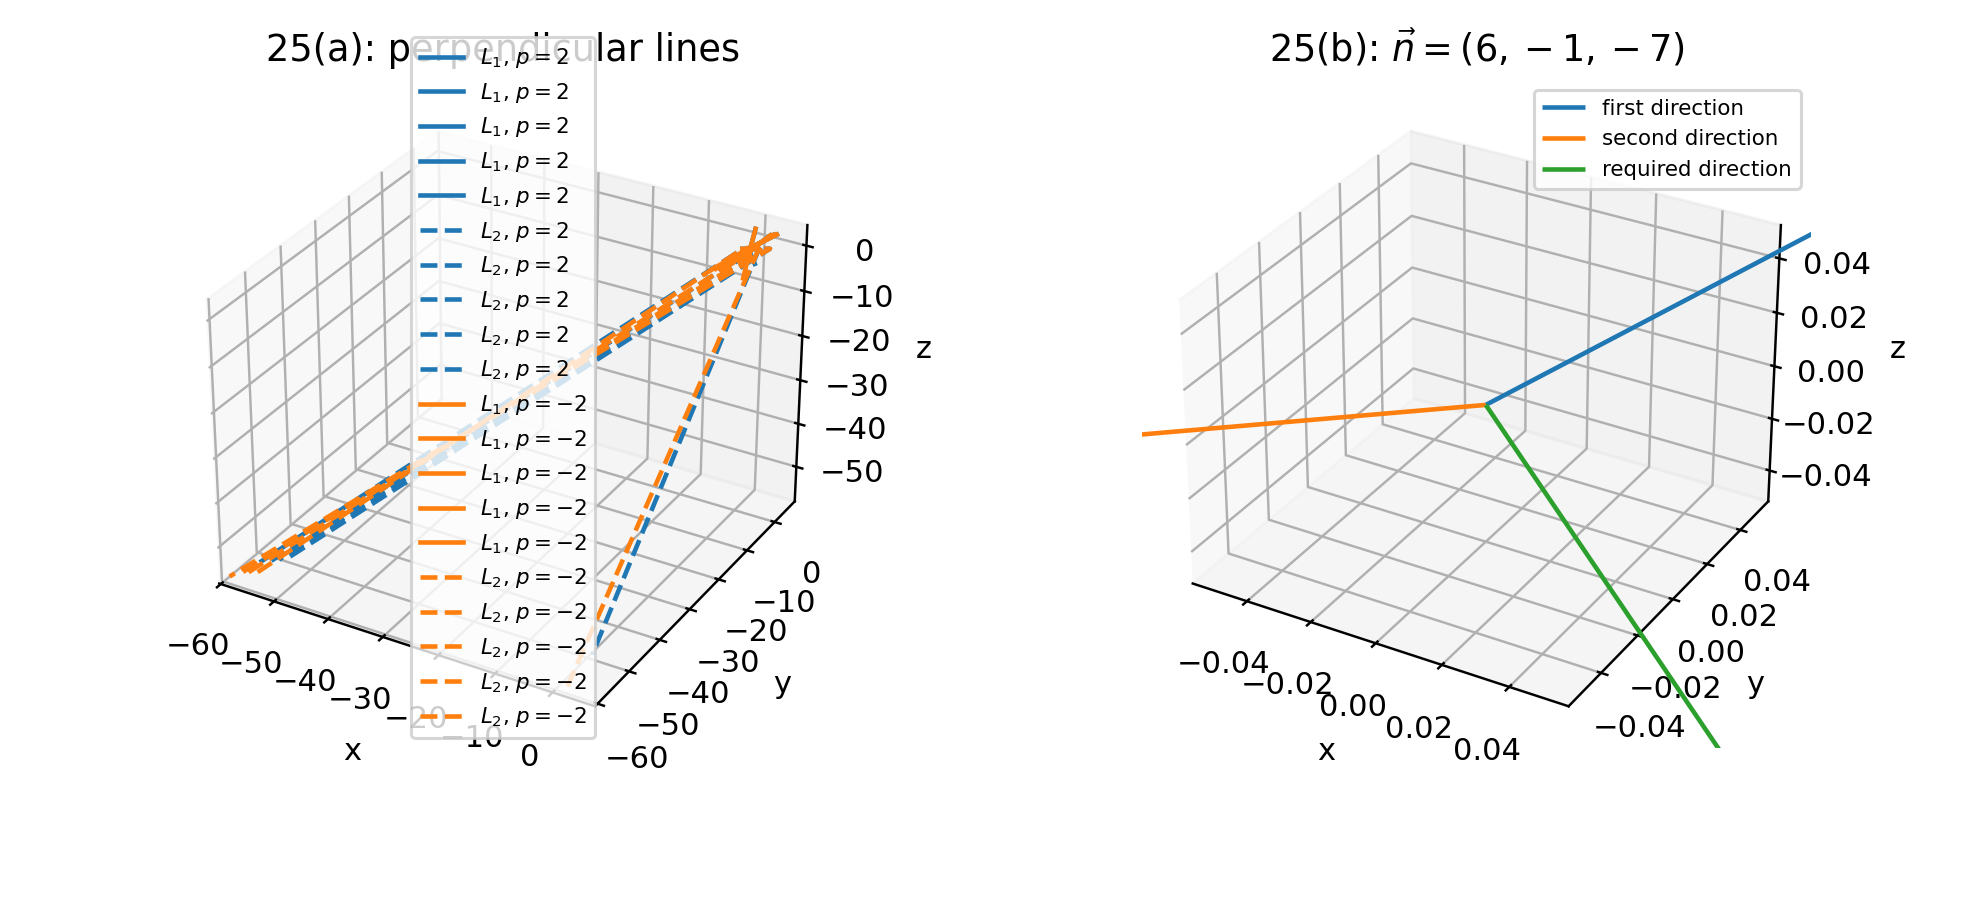
\includegraphics[width=0.75\linewidth]{figs/3.1.25.png}\caption{Direction diagrams for the two alternatives in Question 25.}\end{figure}

\item[3.1.26]
(a) Find $\displaystyle\int\frac{dx}{x^{1/2}+x^{1/3}}$.\\
\textbf{OR}\\
(b) Find $\displaystyle\int\tan^{-1}\!\sqrt{\frac{1-x}{1+x}}\,dx$.

\vspace{0.6em}\par\noindent\textbf{Solution:}

(a) Put $x=t^6$. Then the integral becomes $6\int\frac{t^3}{t+1}\,dt$, giving $\boxed{2\sqrt{x}-3x^{1/3}+6x^{1/6}-6\ln(1+x^{1/6})+C}$.\\
(b) Put $x=\cos\theta$. The radical becomes $\tan(\theta/2)$, and integration by parts gives $\boxed{\frac12x\cos^{-1}x-\frac12\sqrt{1-x^2}+C}$ (on the usual interval $-1<x<1$).

\item[3.1.27] Evaluate $\displaystyle\int_0^\pi\frac{\sin^{2026}x}{\sin^{2026}x+\cos^{2026}x}\,dx$.

\vspace{0.6em}\par\noindent\textbf{Solution:}

The integrand is symmetric about $\pi/2$. On $[0,\pi/2]$, replacing $x$ by $\pi/2-x$ interchanges sine and cosine, so the integral over that half is half the interval length, $\pi/4$. Doubling gives $\boxed{\pi/2}$.

\item[3.1.28]
(a) Find $\displaystyle\int\frac{\cos x}{(2+\sin x)(4+\sin x)}\,dx$.\\
\textbf{OR}\\
(b) Find $\displaystyle\int\frac{x+3}{x^2+4x+5}\,dx$.

\vspace{0.6em}\par\noindent\textbf{Solution:}

(a) With $u=\sin x$, partial fractions give $\boxed{\frac12\ln\left|\frac{2+\sin x}{4+\sin x}\right|+C}$.\\
(b) Write $x+3=\frac12(2x+4)+1$ and complete the square in the denominator. The result is $\boxed{\frac12\ln(x^2+4x+5)+\tan^{-1}(x+2)+C}$.

\item[3.1.29]
(a) Find the general solution of $2x^2\frac{dy}{dx}=y^2+2xy$.\\
\textbf{OR}\\
(b) Find the particular solution of $(x+1)\frac{dy}{dx}=2e^{-y}-1$, given $y=0$ when $x=0$.

\vspace{0.6em}\par\noindent\textbf{Solution:}

(a) For $y=vx$, the equation reduces to $2x\,dv/dx=v^2$. Separating and integrating gives $\boxed{y=0}$ or $\boxed{y=-2x/(\ln|x|+C)}$.\\
(b) Separate variables and integrate to obtain $(x+1)(2-e^y)=C$. The initial condition gives $C=1$, so $\boxed{y=\ln\!\left(2-\frac1{x+1}\right)}$ on the interval where the logarithm is defined.

\item[3.1.30] If $(\sin x)^y=y^{\cos x}$, find $dy/dx$.

\vspace{0.6em}\par\noindent\textbf{Solution:}

Taking logarithms gives $y\ln(\sin x)=\cos x\ln y$. Differentiating implicitly and collecting $y'$ yields
\[
\boxed{\frac{dy}{dx}=\frac{-y\bigl(\sin x\ln y+y\cot x\bigr)}{y\ln(\sin x)-\cos x}}.
\]

\item[3.1.31] Robotic knee replacement surgery has a $90\%$ success rate. For three independent surgeries, find the probability that (i) exactly one succeeds, and (ii) at most two succeed.

\vspace{0.6em}\par\noindent\textbf{Solution:}

With $p=0.9$ and $q=0.1$, (i) $\binom31p q^2=\boxed{0.027}$. (ii) The complement of three successes is $1-p^3=\boxed{0.271}$.

\item[3.1.32] Show that $f:\mathbb R\to\mathbb R$, $f(x)=\frac{x}{\sqrt{1+x^2}}$, is one-one but not onto.

\vspace{0.6em}\par\noindent\textbf{Solution:}

$f'(x)=(1+x^2)^{-3/2}>0$, so $f$ is strictly increasing and therefore one-one. Also $|f(x)|<1$ for every real $x$, and its range is $(-1,1)$, so it is not onto $\mathbb R$. The plot illustrates the range.
\begin{lstlisting}[frame=single, basicstyle=\rmfamily, escapeinside={(*@}{@*)}]
(*@\makebox[\dimexpr\linewidth-2\fboxsep-2\fboxrule\relax][c]{codes/3.1.32.py}@*)
\end{lstlisting}
\begin{figure}[H]\centering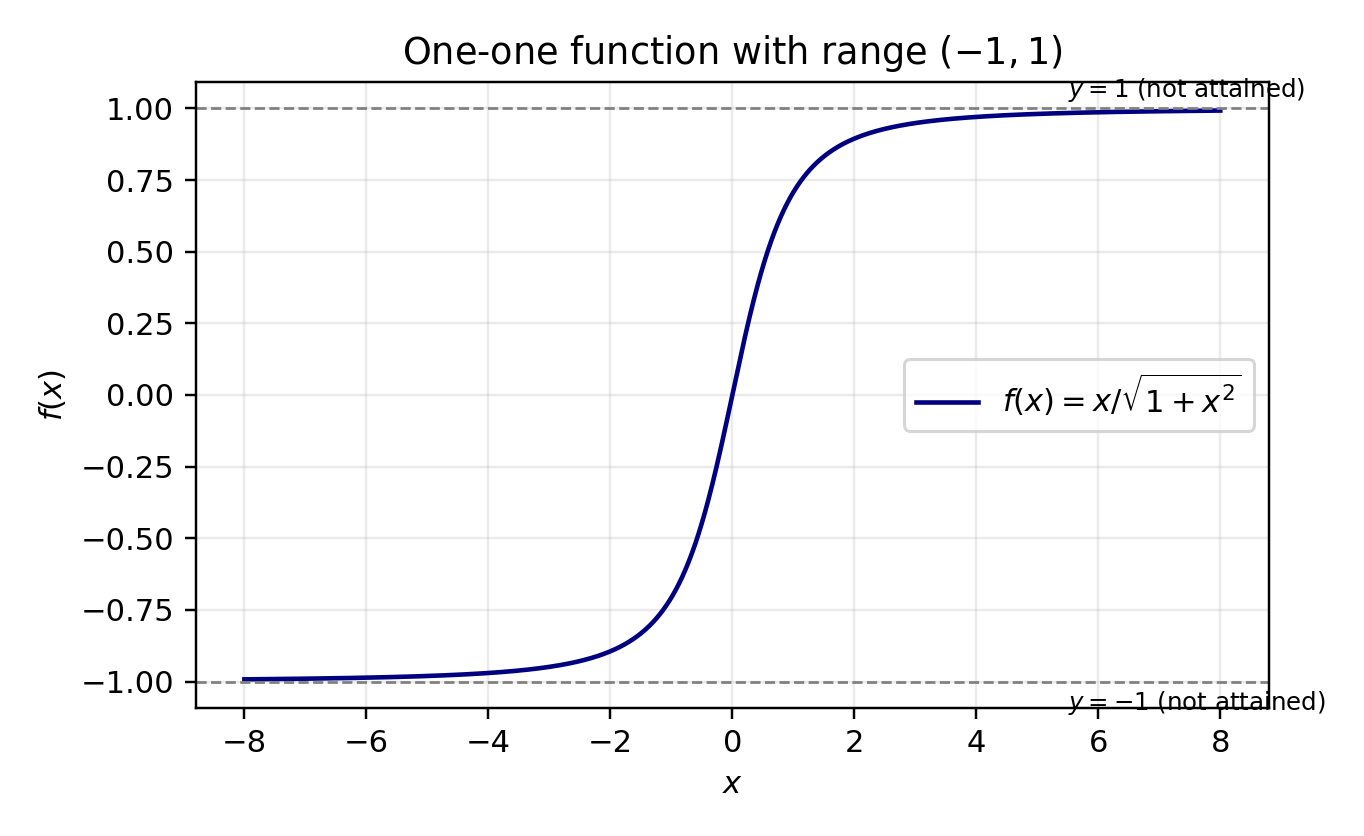
\includegraphics[width=0.68\linewidth]{figs/3.1.32.png}\caption{The function is strictly increasing and approaches, but never reaches, $\pm1$.}\end{figure}

\item[3.1.33] Solve graphically: maximize $Z=600x+400y$ subject to $x+2y\le12$, $4x+5y\ge20$, $2x+y\le12$, and $x,y\ge0$.

\vspace{0.6em}\par\noindent\textbf{Solution:}

The feasible vertices are $(0,4),(0,6),(4,4),(6,0),(5,0)$. Evaluating $Z$ gives $1600,2400,4000,3600,3000$, respectively. Thus $\boxed{Z_{\max}=4000}$ at $(4,4)$. The code plots the constraints and computes each vertex value; it uses CoordGeo line and point-labeling functions.
\begin{lstlisting}[frame=single, basicstyle=\rmfamily, escapeinside={(*@}{@*)}]
(*@\makebox[\dimexpr\linewidth-2\fboxsep-2\fboxrule\relax][c]{codes/3.1.33.py}@*)
\end{lstlisting}
\begin{figure}[H]\centering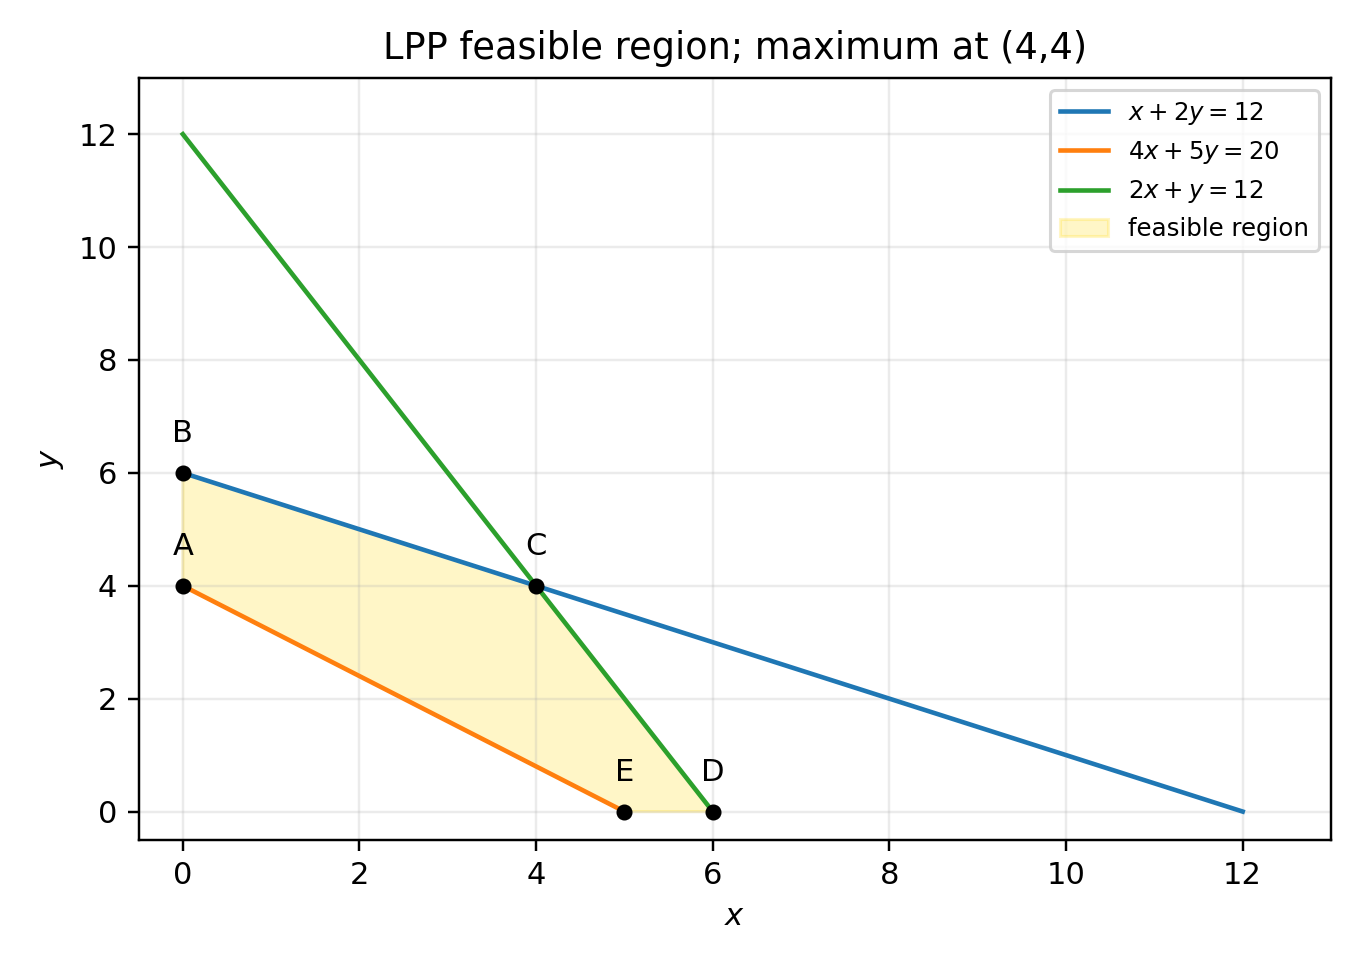
\includegraphics[width=0.68\linewidth]{figs/3.1.33.png}\caption{The shaded feasible region has its maximum at $(4,4)$.}\end{figure}

\item[3.1.34]
(a) A showroom gives 60 vouchers of Rs. 1,000 and Rs. 500. The number of Rs. 1,000 vouchers plus three times the number of Rs. 500 vouchers is 100. Form the equations and find the counts by the matrix method.\\
\textbf{OR}\\
(b) Given $P=\begin{bmatrix}2&-1\\3&4\end{bmatrix}$, $Q=\begin{bmatrix}5&2\\7&4\end{bmatrix}$ and $R=\begin{bmatrix}2&5\\3&8\end{bmatrix}$, find $S$ such that $PQ-RS=O$.

\vspace{0.6em}\par\noindent\textbf{Solution:}

(a) Let $x,y$ denote the two voucher counts. Then $x+y=60$, $x+3y=100$. In matrix form $AX=B$ with $A=\begin{bmatrix}1&1\\1&3\end{bmatrix}$, so $X=A^{-1}B=\begin{bmatrix}40\\20\end{bmatrix}$. There are $\boxed{40}$ Rs. 1,000 vouchers and $\boxed{20}$ Rs. 500 vouchers. Code path: `codes/3.1.34a.py`.\\
(b) $S=R^{-1}PQ$. The Python code evaluates this and verifies $PQ-RS=O$, giving
\[
\boxed{S=\begin{bmatrix}-191&-110\\77&44\end{bmatrix}}.
\]
\begin{lstlisting}[frame=single, basicstyle=\rmfamily, escapeinside={(*@}{@*)}]
(*@\makebox[\dimexpr\linewidth-2\fboxsep-2\fboxrule\relax][c]{codes/3.1.34a.py}@*)
\end{lstlisting}
\begin{lstlisting}[frame=single, basicstyle=\rmfamily, escapeinside={(*@}{@*)}]
(*@\makebox[\dimexpr\linewidth-2\fboxsep-2\fboxrule\relax][c]{codes/3.1.34b.py}@*)
\end{lstlisting}

\item[3.1.35]
(a) Write the lines $\frac{x+3}{-3}=\frac{y-1}{1}=\frac{z-5}{5}$ and $\frac{x+1}{-1}=\frac{2-y}{-2}=\frac{z-5}{5}$ in vector form and check whether they intersect.\\
\textbf{OR}\\
(b) A square has opposite sides along $\vec r=(1,2,-4)+\lambda(2,3,6)$ and $\vec r=(3,3,-5)+\mu(2,3,6)$. If the other pair has direction ratios $(-3,6,p)$, find the square's area and $p$.

\vspace{0.6em}\par\noindent\textbf{Solution:}

(a) The vector forms are $\vec r=(-3,1,5)+\lambda(-3,1,5)$ and $\vec r=(-1,2,5)+\mu(-1,2,5)$. At $\lambda=\mu=-1$, both pass through $(0,0,0)$, so they intersect there.\\
(b) The separation of the parallel lines is $\sqrt{293}/7$, so the square's area is $\boxed{293/49}$. Perpendicular adjacent side directions require $(2,3,6)\cdot(-3,6,p)=0$, giving $\boxed{p=-2}$. The code draws both cases; it uses CoordGeo's line generator for the spatial representation.
\begin{lstlisting}[frame=single, basicstyle=\rmfamily, escapeinside={(*@}{@*)}]
(*@\makebox[\dimexpr\linewidth-2\fboxsep-2\fboxrule\relax][c]{codes/3.1.35.py}@*)
\end{lstlisting}
\begin{figure}[H]\centering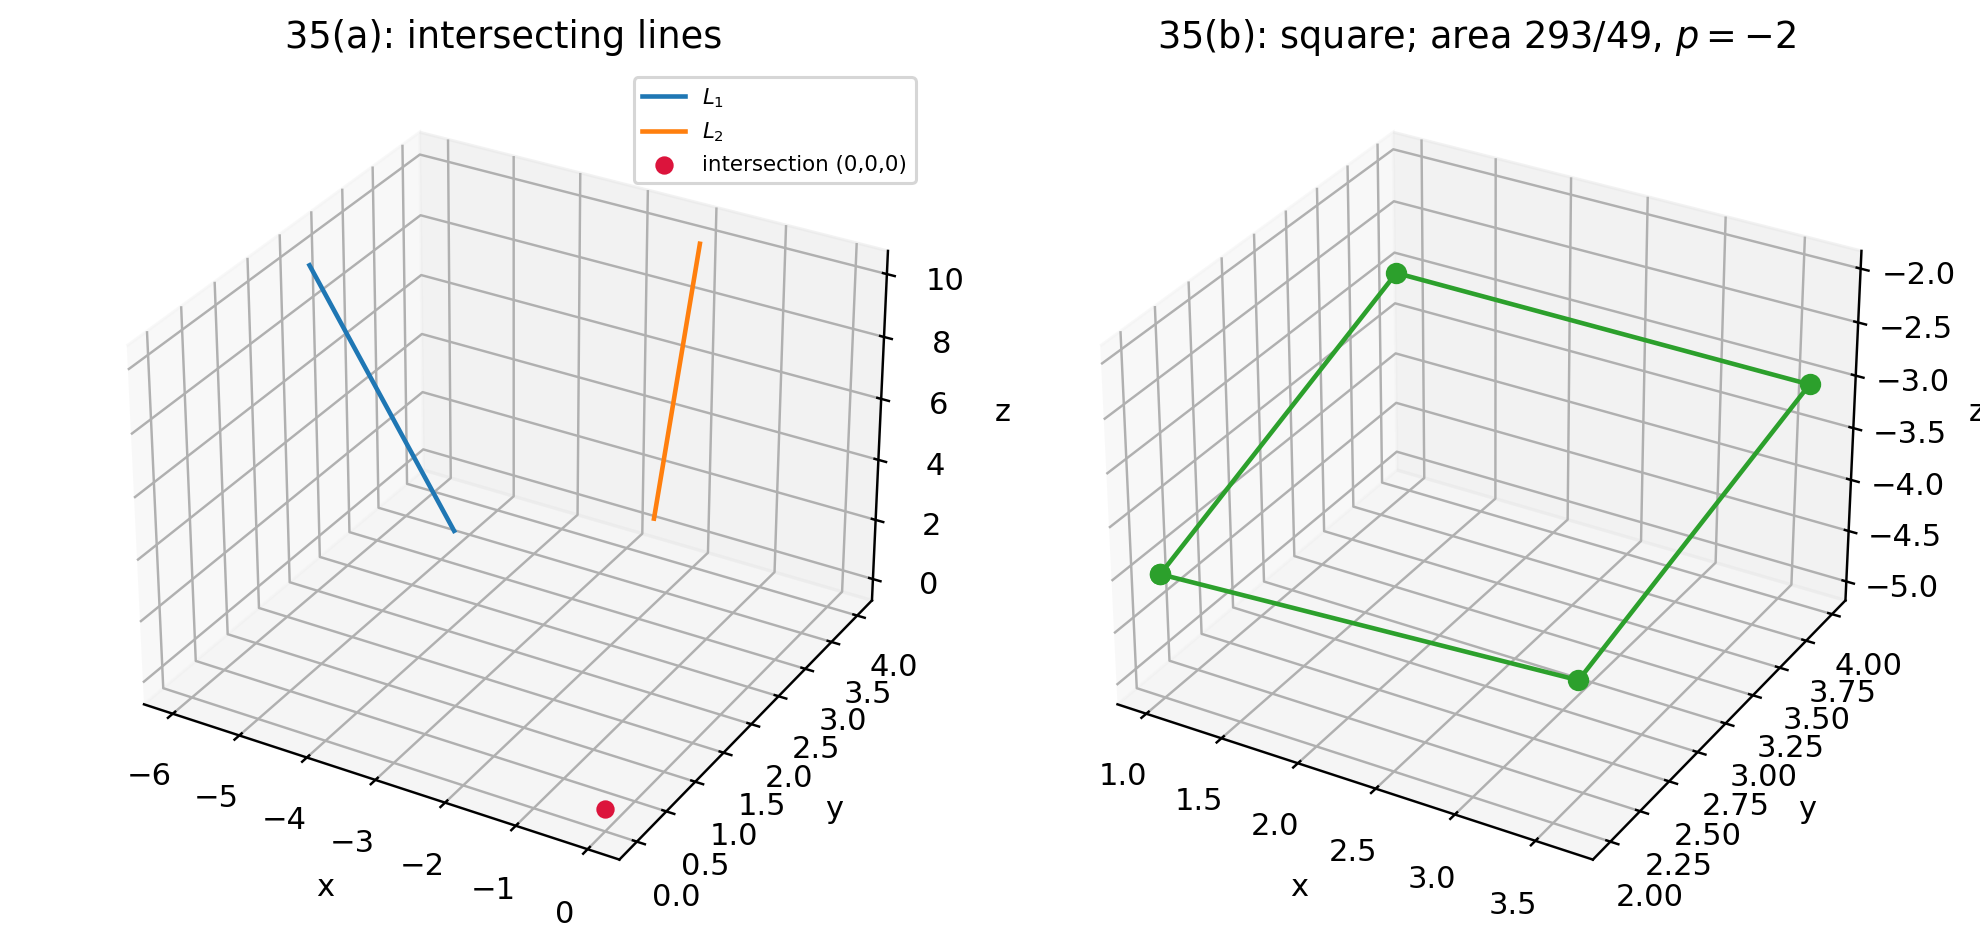
\includegraphics[width=0.75\linewidth]{figs/3.1.35.png}\caption{The two line configurations and the square between parallel lines.}\end{figure}

\item[3.1.36] Two vertical poles of heights $22$ m and $16$ m stand on opposite sides of a $20$ m road. Ladders from a point $R$, $x$ m from the shorter pole, reach their tops. (i) Express $p(x)=l_1+l_2$. (ii) Find $p'(x)$. (iii)(a) Find $x$ minimizing $l_1^2+l_2^2$. \textbf{OR} (b) if both poles are $16$ m tall, find the position minimizing the sum of squared ladder lengths.

\vspace{0.6em}\par\noindent\textbf{Solution:}

The horizontal distances from $R$ to the $22$ m and $16$ m poles are $20-x$ and $x$, respectively. Hence
\[
\begin{aligned}
l_1(x)&=\sqrt{484+(20-x)^2}, & l_2(x)&=\sqrt{256+x^2},\\
p(x)&=l_1+l_2=\sqrt{484+(20-x)^2}+\sqrt{256+x^2},\\
p'(x)&=-\frac{20-x}{\sqrt{484+(20-x)^2}}+\frac{x}{\sqrt{256+x^2}}.
\end{aligned}
\]
For (a),
\[
l_1^2+l_2^2=484+(20-x)^2+256+x^2=2(x-10)^2+940,
\]
so the minimum occurs at $\boxed{x=10\text{ m}}$.
For (b), if both poles are $16$ m tall, the sum of squared ladder lengths is
\[
[256+(20-x)^2]+[256+x^2]=2(x-10)^2+712,
\]
which is minimized when $\boxed{x=10\text{ m}}$, the midpoint of the road.

\newpage
\item[3.1.37] Of students taking an entrance examination, $40\%$ are dropouts and $60\%$ are regular students. The pass rates are $5\%$ for dropouts and $10\%$ for regular students. Find (i) the probability a student is regular, (ii) the probability a dropout fails, (iii)(a) given a student passed, the probability they are not a dropout, \textbf{OR} (b) given a student failed, the probability they were regular.

\vspace{0.6em}\par\noindent\textbf{Solution:}

Let $D$ denote dropout, $R$ regular, $S$ pass, and $F$ fail. Then $P(D)=0.4$, $P(R)=0.6$, $P(S\mid D)=0.05$, and $P(S\mid R)=0.10$.
\begin{align*}
\text{(i)}\quad&P(R)=\boxed{0.6}.\\
\text{(ii)}\quad&P(F\mid D)=1-P(S\mid D)=1-0.05=\boxed{0.95}.\\[2pt]
\text{(iii)(a)}\quad&P(R\mid S)=\frac{P(R)P(S\mid R)}{P(D)P(S\mid D)+P(R)P(S\mid R)}\\
&=\frac{0.6(0.10)}{0.4(0.05)+0.6(0.10)}=\frac{0.06}{0.08}=\boxed{\frac34}.\\[2pt]
\text{(iii)(b)}\quad&P(R\mid F)=\frac{P(R)P(F\mid R)}{P(D)P(F\mid D)+P(R)P(F\mid R)}\\
&=\frac{0.6(0.90)}{0.4(0.95)+0.6(0.90)}=\frac{0.54}{0.92}=\boxed{\frac{27}{46}}.
\end{align*}

\item[3.1.38] A triangular park has vertices $A(0,4)$, $B(-2,0)$ and $C(3,0)$, with $O=(0,0)$. Find (i) the equation of $AB$, (ii) the equation of $AC$, and (iii)(a) the area of $OAC$ by integration, \textbf{OR} (b) the area of $AOB$ by integration.

\vspace{0.6em}\par\noindent\textbf{Solution:}

The line through $A,B$ is $\boxed{y=2x+4}$ and the line through $A,C$ is $\boxed{y=4-\frac43x}$. (iii)(a) $\int_0^3(4-\frac43x)\,dx=\boxed{6}$ square units. (iii)(b) $\int_{-2}^0(2x+4)\,dx=\boxed{4}$ square units.
\end{list}

\end{document}
